\documentclass[10pt,a4paper]{article}
\usepackage[utf8]{inputenc}
\usepackage[T1]{fontenc}
\usepackage{amsmath}
\usepackage{amssymb}
\usepackage{graphicx}
\graphicspath{{images/}}
\usepackage{pdfpages}
\usepackage{caption, subcaption}
\usepackage{booktabs}
\usepackage{multirow, multicol}
\usepackage{listings}
\usepackage{xcolor}
\definecolor{codegreen}{rgb}{0,0.6,0}
\definecolor{codegray}{rgb}{0.5,0.5,0.5}
\definecolor{codepurple}{rgb}{0.58,0,0.82}
\definecolor{backcolour}{rgb}{0.95,0.95,0.92}
\definecolor{codenavy}{rgb}{0,0,0.8}
\lstdefinestyle{mystyle}{
	backgroundcolor=\color{backcolour},   
	commentstyle=\color{codegreen},
	keywordstyle=\color{codenavy},
	numberstyle=\tiny\color{codegray},
	stringstyle=\color{codepurple},
	basicstyle=\ttfamily\footnotesize,
	breakatwhitespace=false,         
	breaklines=true,                 
	captionpos=b,                    
	keepspaces=true,                 
	numbers=left,                    
	numbersep=5pt,                  
	showspaces=false,                
	showstringspaces=false,
	showtabs=false,                  
	tabsize=2
}
\lstset{style=mystyle}
\title{{\LARGE SAS Project}}
\author{ {\LARGE Jesse Annan \hspace{0.5cm} | \hspace{0.5cm} ID: 002708111 }}

\begin{document}
	\maketitle
	\sffamily
	\clearpage
	
	\begin{enumerate}
		\item \textbf{Question 1: Descriptive Statistics} \newline
			\begin{enumerate}
				\item[(a)] MLB2009-AL.xls
					\begin{figure}[h!]
						\centering
						\begin{subfigure}{0.49\textwidth}
							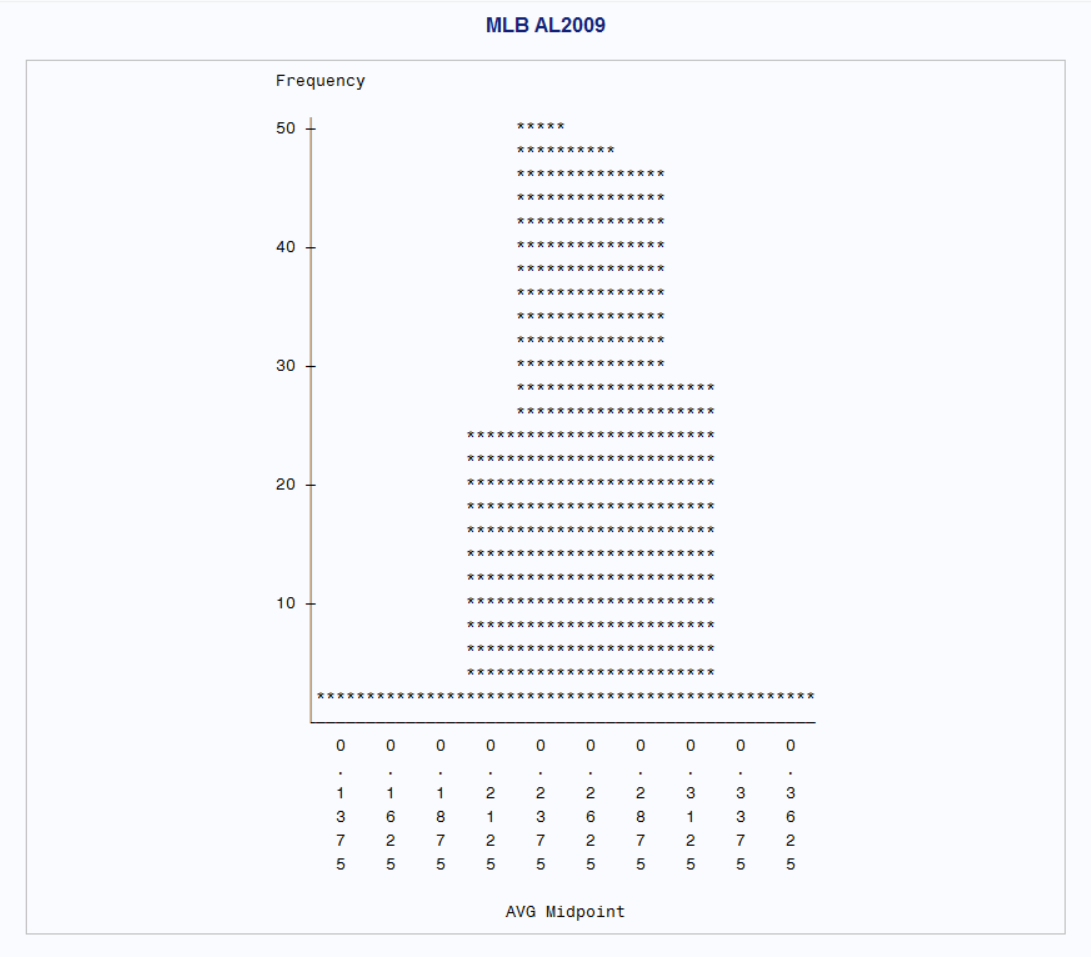
\includegraphics[width=\textwidth]{hist_al2009}
							\caption{Histogram}
						\end{subfigure}
						\hfill
						\begin{subfigure}{0.49\textwidth}
							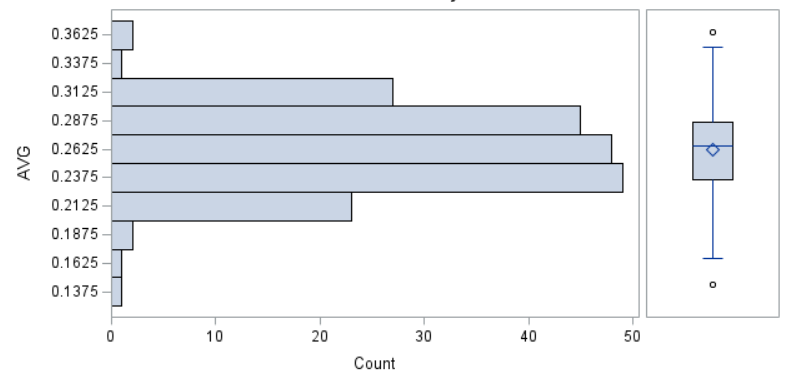
\includegraphics[width=\textwidth]{sal_al2009}
							\caption{Stem-and-Leaf plot}
						\end{subfigure}
					\end{figure}
					
					Looking at the histogram and stem-and-leaf plots we can conclude that the data points are close to the sample mean and it also looks like the data is from a normal probability distribution. \vspace*{1cm}
				
				\item[(b)] MLB2009-NL.xls
					\begin{figure}[h!]
						\centering
						\begin{subfigure}{0.49\textwidth}
							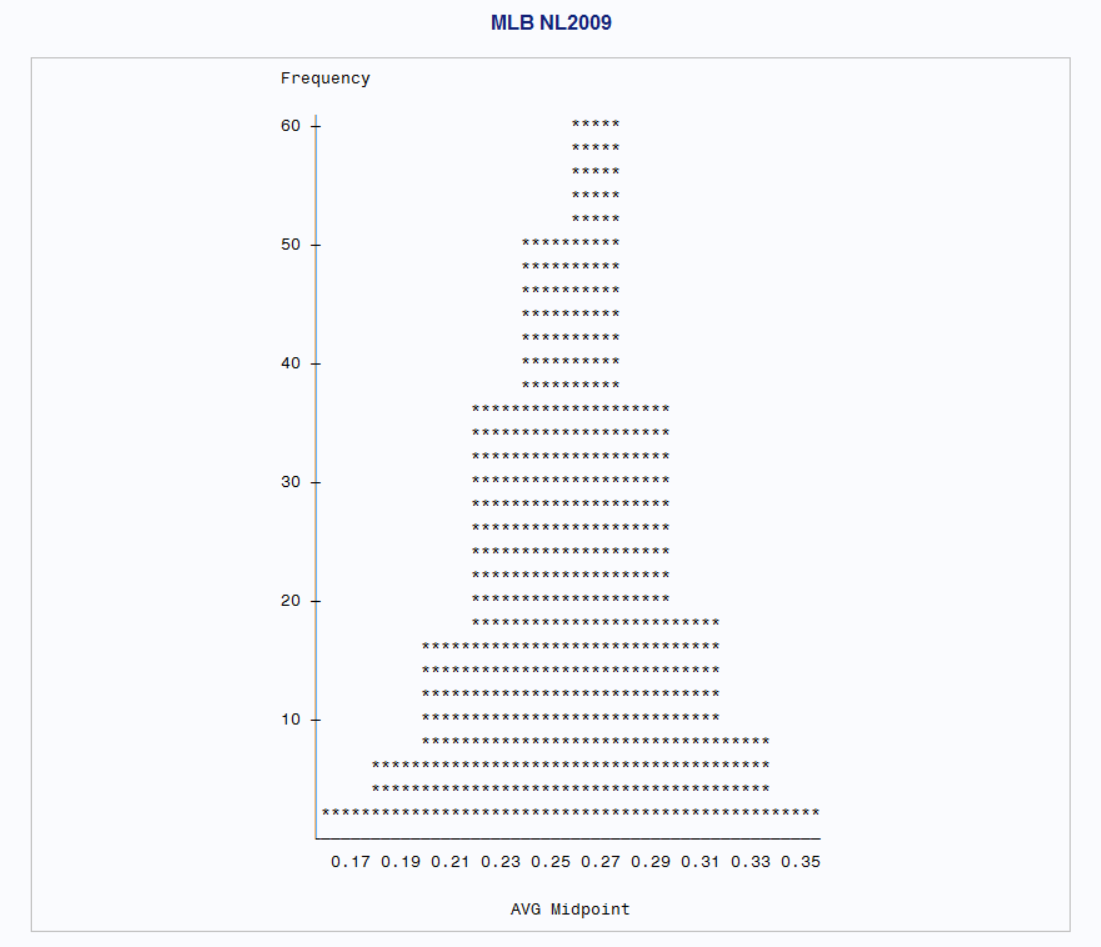
\includegraphics[width=\textwidth]{hist_nl2009}
							\caption{Histogram}
						\end{subfigure}
						\hfill
						\begin{subfigure}{0.49\textwidth}
							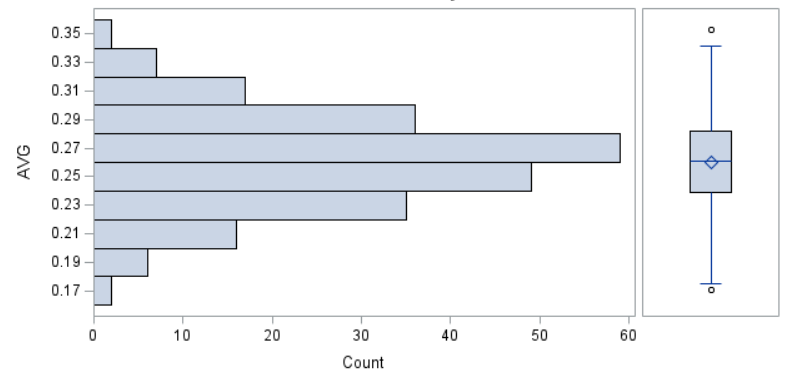
\includegraphics[width=\textwidth]{sal_nl2009}
							\caption{Stem-and-Leaf plot}
						\end{subfigure}
					\end{figure}
				
					Looking at the histogram and stem-and-leaf plots we can conclude that the data is from a normal probability distribution because of the bell shape of both descriptive statistics.
					
			\end{enumerate}
		
		\clearpage
		\item \textbf{Question 2: Intervals and Percentage of Measurements} \newline
			\begin{enumerate}
				\item[(a)] MLB2009-AL.xls
					\begin{figure}[h!]
						\centering
						\begin{subfigure}{0.49\textwidth}
							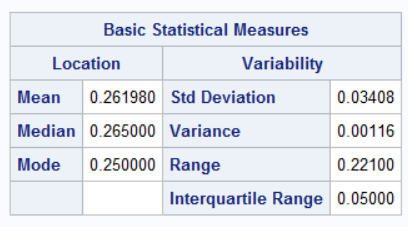
\includegraphics[width=\textwidth]{mean_al2009}
							\caption{Histogram}
						\end{subfigure}
						\hfill
						\begin{subtable}{0.49\textwidth}
							\begin{tabular}{cccc}
								\multicolumn{2}{c}{Ranges} & Count & \% \\ \toprule
								$ \bar{x} \pm s $ & ( 0.22790, 0.29606 ) & 133 & 66.83 \\
								$ \bar{x} \pm 2s $ & ( 0.19381, 0.33015 ) & 192 & 96.48 \\
								$ \bar{x} \pm 3s $ & ( 0.15973, 0.36423 ) & 197 & 98.99 \\ \bottomrule
							\end{tabular}
							\caption{Intervals and \% of Measurements}
						\end{subtable}
					\end{figure}
				
					The \%s are fairly close to the empirical rule and thus we can say the data is approximately symmetric, with clustering of measurements about the midpoint of the distribution. \vspace*{0.5cm}				
				
				\item[(b)] MLB2009-NL.xls
					\begin{figure}[h!]
						\centering
						\begin{subfigure}{0.49\textwidth}
							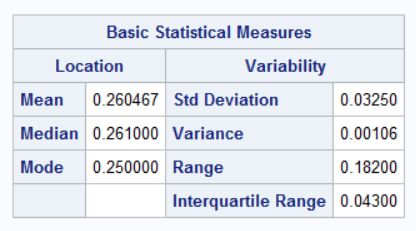
\includegraphics[width=\textwidth]{mean_nl2009}
							\caption{Histogram}
						\end{subfigure}
						\hfill
						\begin{subtable}{0.49\textwidth}
							\begin{tabular}{cccc}
								\multicolumn{2}{c}{Ranges} & Count & \% \\ \toprule
								$ \bar{x} \pm s $ & ( 0.22797, 0.29296 ) & 160 & 69.87 \\
								$ \bar{x} \pm 2s $ & ( 0.19548, 0.32546 ) & 217 & 94.76 \\
								$ \bar{x} \pm 3s $ & ( 0.16298, 0.35796 ) & 229 & 100.00 \\ \bottomrule
							\end{tabular}
							\caption{Intervals and \% of Measurements}
						\end{subtable}
					\end{figure}
				
					The \%s are quite close to the empirical rule and thus we can say the data is approximately symmetric, with clustering of measurements about the midpoint of the distribution. \vspace*{1cm}
					
			\end{enumerate}
		
		
		\item \textbf{Question 3: IQR/s} \newline
			\begin{enumerate}
				\item[MLB2009-AL: ] $ \frac{IQR}{s} = \frac{0.05}{0.03408} \approx 1.46695 $ \newline
				Since this value is a bit bigger than 1.3, we may conclude that the data are not approximately normal. \vspace*{0.5cm}
				
				\item[MLB2009-NL: ] $ \frac{IQR}{s} = \frac{0.043}{0.0325} \approx 1.32324 $ \newline
				Since this value is approximately equal to 1.3, we have further confirmation that the data are approximately normal.
			\end{enumerate}
			
			
			\clearpage
		\item \textbf{Question 4: Normal Probability Plots} \newline
			\begin{figure}[h!]
				\centering
				\begin{subfigure}{0.49\textwidth}
					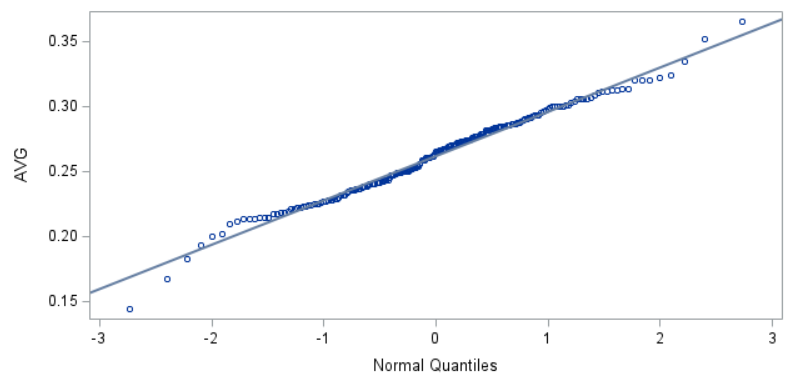
\includegraphics[width=\textwidth]{normal_al2009}
					\caption{Normal Plot for MLB-AL2009}
				\end{subfigure}
				\hfill
				\begin{subfigure}{0.49\textwidth}
					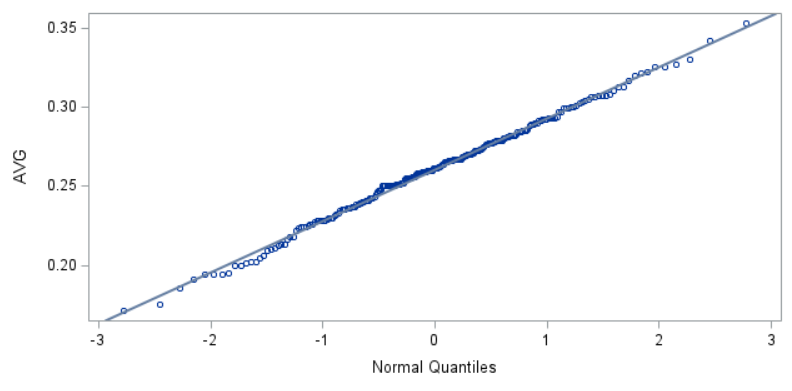
\includegraphics[width=\textwidth]{normal_nl2009}
					\caption{Normal plot for MLB-NL2009}
				\end{subfigure}
			\end{figure}
			
			Its very clear that the AVG values fall reasonably close to the straight line for both data set and thus it suggest that both data set are approximately normally distributed. \vspace*{1cm}
		
		\item \textbf{Question 5: Summary} \newline
			In this project I used SAS programming language to determine whether the data from \textit{MLB2009-AL} and \textit{MLB2009-NL} are from an approximately normal distribution. Checks 1 through 4 on the \textit{MLB2009-NL} satisfied the respective rules and thus it is reasonable to believe that the data are from a normal distribution. On the other hand, \textit{MLB2009-AL}, suggests that the data is from a normal distribution based on Checks 1, 2, and 4. \newline
			Check 3, provides doubt that the data is from a normal distribution since the ratio, $ IQR/s \approx 1.46695 $, is quite greater than $ 1.3 $. 
		
	\end{enumerate}
	
	\clearpage
	
	\begingroup
	\section{\texttt{CODE FOR MLB2009-AL.xls}}
		\lstinputlisting[language=SAS]{sasproject_al2009.sas}
		\includepdf[pages=6-]{mlb_al2009.pdf}
	\endgroup
	
	%\clearpage
	
	\begingroup
		\section{\texttt{CODE FOR MLB2009-NL.xls}}
		\lstinputlisting[language=SAS]{sasproject_nl2009.sas}
		\includepdf[pages=7-]{mlb_nl2009.pdf}
	\endgroup
\end{document}